% ============================================================
%  IEEE Journal Paper — Intracranial Aneurysm Detection
%  Template: IEEEtran (journal mode)
%  Compile:  pdflatex -> bibtex -> pdflatex -> pdflatex
% ============================================================
\documentclass[journal]{IEEEtran}

% ── Packages ─────────────────────────────────────────────────
\usepackage[T1]{fontenc}
\usepackage[utf8]{inputenc}
\usepackage{amsmath,amssymb}
\usepackage{graphicx}
\usepackage{booktabs}
\usepackage{multirow}
\usepackage{array}
\usepackage{cite}
\usepackage{url}
\usepackage{xcolor}
\usepackage{float}
\usepackage{balance}       % balance last-page columns
\usepackage{hyperref}
\hypersetup{colorlinks=true,linkcolor=blue,citecolor=blue,urlcolor=blue}
\pagestyle{empty}

% ── Title & Authors ──────────────────────────────────────────
\title{Automated Intracranial Aneurysm Detection Using 3-D Residual Encoder U-Net\\
       with EDT Blob Regression and Vision-Language Model Analysis}

\author{\IEEEauthorblockN{Muahmmed Rayan*, Alen Sebastian\textsuperscript{\textdagger}, Tobin Tom\textsuperscript{\textdaggerdbl}, Ajas Ajmal\textsuperscript{\textsection}, Subash M\textsuperscript{\textparagraph}, Athira S Nath\textsuperscript{\textbar}, Dr. Ojus Thomas Lee\textsuperscript{\#}}
\IEEEauthorblockA{\textit{Department of CSE, College of Engineering Kidangoor} \\
\textit{Kottayam, Kerala, India}\\
*rayan6203@gmail.com, \textsuperscript{\textdagger}alenvattakunnel6@gmail.com, \textsuperscript{\textdaggerdbl}tobintom222@gmail.com, \\
\textsuperscript{\textsection}ajasajmal03@gmail.com, \textsuperscript{\textparagraph}sm29032004@gmail.com, \textsuperscript{\textbar}athiranath695@gmail.com, \textsuperscript{\#}ojusthomaslee@gmail.com}
}
% ── Begin Document ───────────────────────────────────────────
\begin{document}

\maketitle
\thispagestyle{empty}

% ────────────────────────────────────────────────────────────
\begin{abstract}
Intracranial aneurysms (IAs) are focal dilations of cerebral arteries that
affect an estimated 3--5\% of the adult population and carry a mortality
rate exceeding 50\% upon rupture. Reliable automated detection from
multi-modality neuroimaging remains an open challenge due to the small size
of lesions, high anatomical variability, and the diversity of imaging
protocols. This paper presents a dual-model deep-learning framework that
simultaneously investigates two complementary approaches for IA detection and
anatomical localization across 13 cerebrovascular regions. The first model is a
\textbf{3-D Residual Encoder U-Net} built on the nnU-Net self-configuring
framework, employing a novel \emph{blob regression} strategy that generates
14 volumetric heatmaps instead of bounding boxes, where peak-voxel intensity
encodes aneurysm presence and 3-D coordinates. The model is trained for 1,500
epochs on 4,348 multi-modality series from the RSNA 2025 Intracranial Aneurysm
Detection dataset using TopK Binary Cross-Entropy loss and SGD with polynomial
learning rate decay. The second model is \textbf{MedGemma 4B-it}, Google's
open-source multimodal medical vision-language model, applied with
modality-specific image windowing, structured chain-of-thought prompting, and
BiomedCLIP confidence ensembling across a multi-slice context window. Both
models are independently evaluated using sensitivity, specificity, precision,
F1 score, and Dice similarity coefficient at series and anatomical-location
levels. Our results demonstrate that the volumetric CNN achieves superior
spatial precision while the vision-language model provides interpretable
natural-language findings, establishing complementary strengths suitable for
a research-grade clinical decision-support context.
\end{abstract}

\begin{IEEEkeywords}
Intracranial aneurysm, subarachnoid hemorrhage, nnU-Net, medical image
segmentation, vision-language model, MedGemma, blob regression, heatmap
detection, DICOM, neuroimaging.
\end{IEEEkeywords}

% ════════════════════════════════════════════════════════════
\section{Introduction}
\label{sec:intro}
% ════════════════════════════════════════════════════════════

Intracranial aneurysms are pathological bulges of the cerebral arterial wall
that form predominantly at bifurcation points of the Circle of Willis.
While the majority of aneurysms remain clinically silent throughout a patient's
lifetime, rupture precipitates subarachnoid hemorrhage (SAH), a devastating
neurological emergency. Population-based studies estimate a prevalence of
3--5\% in the general adult population~\cite{rinkel1998prevalence}, yet the
condition consistently escapes detection prior to rupture owing to the absence
of prodromal symptoms.

The clinical and socioeconomic burden of IA is disproportionately severe.
Following rupture, 30-day mortality reaches 40--50\%; of survivors,
approximately 30\% suffer permanent neurological disability~\cite{feigin2009}.
Even unruptured aneurysms, once incidentally discovered, create significant
patient anxiety and necessitate careful monitoring or prophylactic intervention.

Standard diagnostic approaches rely on CT angiography (CTA), MR angiography
(MRA), and digital subtraction angiography (DSA). Neuroradiologists manually
review hundreds of cross-sectional slices to identify lesions that can be
as small as 2--3 mm in diameter, a process that is time-intensive and
subject to inter-reader variability. Studies have shown that small aneurysms
($<$ 5 mm) are missed in up to 28\% of cases on initial reading~\cite{white2001}.

Recent advances in 3-D convolutional neural networks (CNNs) and the emergence
of large multimodal language models have opened new avenues for automated
detection. Architectures such as U-Net~\cite{unet2015} and nnU-Net~\cite{nnunet2021},
together with self-attention mechanisms, have demonstrated competitive
performance on several medical segmentation benchmarks. Consequently, various studies
have successfully applied deep learning and computational modeling for
IA detection tasks~\cite{yang2021, lauric2010, ueda2019, bizjak2023}.

Contributions of our works are:
\begin{itemize}
  \item A \textbf{blob regression} formulation for IA detection that replaces
        standard bounding-box heads with smooth volumetric heatmaps, better
        matching the spherical geometry of aneurysms.
  \item End-to-end evaluation of \textbf{MedGemma 4B-it} as a zero-shot
        medical vision-language model for IA detection on a large-scale
        benchmark dataset.
  \item A \textbf{comparative analysis} of both approaches across four imaging
        modalities and 13 anatomical locations, establishing their respective
        strengths and failure modes.
  \item A \textbf{memory-efficient evaluation pipeline} capable of processing
        4,348 DICOM series directly from a compressed archive without disk
        extraction overhead.
\end{itemize}

% ════════════════════════════════════════════════════════════
\section{Medical Background}
\label{sec:medical}
% ════════════════════════════════════════════════════════════

\subsection{Intracranial Aneurysm Pathophysiology}

An intracranial aneurysm develops when degenerative changes weaken the arterial
wall at a point of high haemodynamic stress, typically a vessel bifurcation.
The weakened media and internal elastic lamina allow the vessel to balloon
outward, forming saccular (berry), fusiform, or dissecting aneurysm types.
Saccular aneurysms account for 80--85\% of all IAs and are the most clinically
significant owing to their propensity for rupture.

Risk factors include hypertension, cigarette smoking, female sex, family history,
and connective tissue disorders such as Ehlers-Danlos syndrome and autosomal
dominant polycystic kidney disease~\cite{rinkel1998prevalence}. Incidence peaks
in the fifth and sixth decades of life, consistent with the age distribution
observed in the dataset used for this study (mean age 58.5 years).

\subsection{Anatomical Locations}

The Circle of Willis and its branches constitute the principal sites of
aneurysm formation. Clinically significant locations include:

\begin{itemize}
  \item \textbf{Anterior communicating artery (AComA):} Most common location,
        accounting for approximately 30--35\% of all IAs.
  \item \textbf{Internal carotid artery (ICA):} Including both infraclinoid
        and supraclinoid segments; collectively the second most frequent site.
  \item \textbf{Middle cerebral artery (MCA):} Bifurcation aneurysms
        constitute roughly 15--20\% of cases.
  \item \textbf{Posterior communicating artery (PComA):} Associated with
        oculomotor nerve palsy when large.
  \item \textbf{Basilar artery tip and posterior circulation:} Less common but
        surgically more challenging.
\end{itemize}

Table~\ref{tab:locations} summarises the 13 anatomical targets used in this
study and their frequency in the dataset.

\begin{table}[H]
\renewcommand{\arraystretch}{1.3}
\caption{Aneurysm Location Distribution in the RSNA 2025 Dataset}
\label{tab:locations}
\centering
\begin{tabular}{lcc}
\toprule
\textbf{Anatomical Location} & \textbf{Count} & \textbf{\% of Positives} \\
\midrule
Anterior Communicating Artery          & 363 & 19.5 \\
L. Supraclinoid ICA                    & 331 & 17.8 \\
R. Middle Cerebral Artery              & 294 & 15.8 \\
R. Supraclinoid ICA                    & 277 & 14.9 \\
L. Middle Cerebral Artery              & 219 & 11.8 \\
Other Posterior Circulation            & 113 &  6.1 \\
Basilar Tip                            & 110 &  5.9 \\
R. Posterior Communicating Artery      & 101 &  5.4 \\
R. Infraclinoid ICA                    &  98 &  5.3 \\
L. Posterior Communicating Artery      &  86 &  4.6 \\
L. Infraclinoid ICA                    &  78 &  4.2 \\
R. Anterior Cerebral Artery            &  56 &  3.0 \\
L. Anterior Cerebral Artery            &  46 &  2.5 \\
\bottomrule
\end{tabular}
\end{table}

\subsection{Imaging Modalities}

\textbf{CT Angiography (CTA)} is the workhorse modality for IA detection in
emergency settings. Iodinated contrast is administered intravenously, and rapid
helical acquisition produces isotropic voxels at 0.5--0.6 mm spacing.
CTA provides excellent spatial resolution and wide availability but involves
ionising radiation.

\textbf{MR Angiography (MRA)} uses time-of-flight or phase-contrast techniques
without ionising radiation or contrast agents, making it preferable for
screening and follow-up. MRA is susceptible to flow-related signal loss and
has slightly lower spatial resolution than CTA.

\textbf{MRI T1 Post-contrast} and \textbf{MRI T2} sequences are used
adjunctively to characterise the aneurysm wall, detect intraluminal thrombus,
and assess peri-aneurysmal oedema as markers of rupture risk.



% ════════════════════════════════════════════════════════════
\section{Dataset}
\label{sec:dataset}
% ════════════════════════════════════════════════════════════

\subsection{RSNA 2025 Intracranial Aneurysm Detection Dataset}

The dataset used in this study is the RSNA 2025 Intracranial Aneurysm Detection
challenge dataset, hosted on Kaggle~\cite{rsna2025}. It comprises \textbf{4,348
multi-modality DICOM series} from multiple imaging sites, representing one of the
largest publicly available annotated IA datasets to date.

\subsection{Class Distribution}

Of the 4,348 series, 1,864 (42.9\%) are labelled as positive for at least one
aneurysm at one or more anatomical locations, and 2,484 (57.1\%) are negative ---
a moderate class imbalance that informed the choice of TopK Binary Cross-Entropy
as the training objective.

\subsection{Modality Breakdown}

The dataset spans four imaging modalities:
\begin{itemize}
  \item \textbf{CTA:} 1,808 series (41.6\%)
  \item \textbf{MRA:} 1,252 series (28.8\%)
  \item \textbf{MRI T2:}  983 series (22.6\%)
  \item \textbf{MRI T1 Post-contrast:} 305 series (7.0\%)
\end{itemize}

\subsection{Patient Demographics}

The dataset spans patients aged 18 to 89 years (mean 58.5, median 59.0).
Female patients constitute 69.1\% (3,005 series), consistent with the
well-established epidemiological female predominance of intracranial aneurysms.

\subsection{Dataset Fingerprint and Intensity Statistics}

Dataset fingerprinting, as implemented by nnU-Net, revealed a foreground
Hounsfield unit (HU) range of $[-11{,}140,\;+13{,}513]$ with mean $+33.8$ HU,
standard deviation 1,461 HU, and a 99.5th percentile of $+5,511$ HU.
Normalization truncates at the 0.5th and 99.5th percentiles before applying
z-score normalization, effectively suppressing metal-implant and air-cavity
artefacts while preserving the contrast between blood-filled vasculature
and surrounding brain parenchyma.

% ════════════════════════════════════════════════════════════
\section{Methodology}
\label{sec:method}
% ════════════════════════════════════════════════════════════

\subsection{System Overview}

The proposed framework consists of four sequential stages, as illustrated
in Fig.~\ref{fig:architecture}: (1) DICOM ingestion and modality
detection, (2) modality-specific preprocessing and ROI cropping,
(3) dual-model inference, and (4) result aggregation and evaluation.

\begin{figure}[!t]
\centering
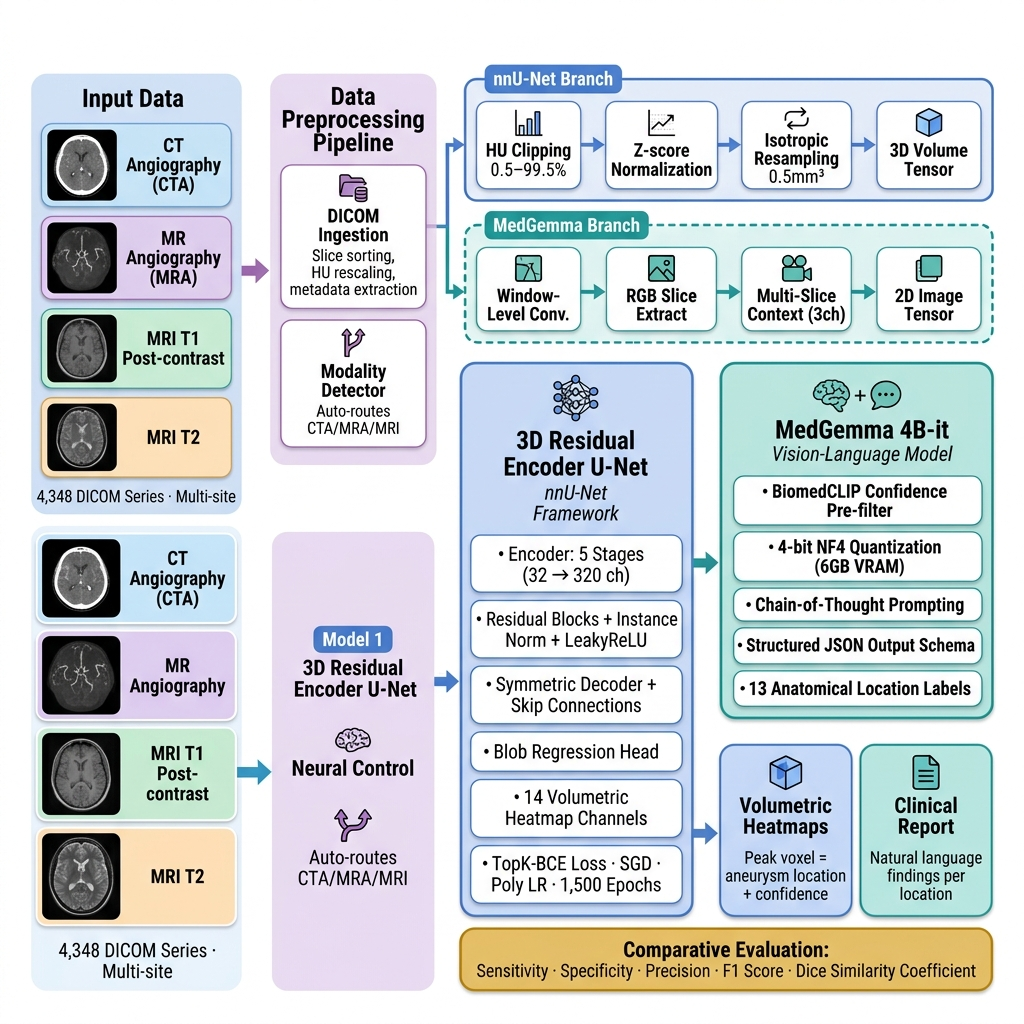
\includegraphics[width=\columnwidth]{figures/architecture.png}
\caption{End-to-end architecture of the proposed dual-model framework for
intracranial aneurysm detection. DICOM series undergo modality-specific
preprocessing before being routed to the nnU-Net volumetric branch and the
MedGemma vision-language branch independently.}
\label{fig:architecture}
\end{figure}

\subsection{Data Preprocessing Pipeline}

\subsubsection{DICOM Ingestion and Orientation}
Raw DICOM series are converted to NIfTI format using \texttt{pydicom},
processing 2-D DICOM slices in parallel. Spacing, origin, and direction
cosines are extracted from the DICOM header and the resulting volume is
wrapped in a SimpleITK image oriented in RAS (Right-Anterior-Superior)
coordinate convention. Series presenting strong artefacts such as completely
empty volumes or unrecoverable orientation defects are discarded; series
with mild mis-orientations are corrected via axis flipping. In total, ten
volumes were discarded from the training set.

\subsubsection{Region-of-Interest Cropping}
To reduce computational cost, a fixed $200 \times 160 \times 160$\;mm
cuboid Region of Interest (ROI) is extracted from the central superior
region of each volume, centred on the Circle of Willis. All aneurysm
annotations in the training set were verified to fall within this ROI.
Fig.~\ref{fig:roi} illustrates the ROI boundary overlaid on axial, coronal,
and sagittal CT views.

\begin{figure}[!t]
\centering
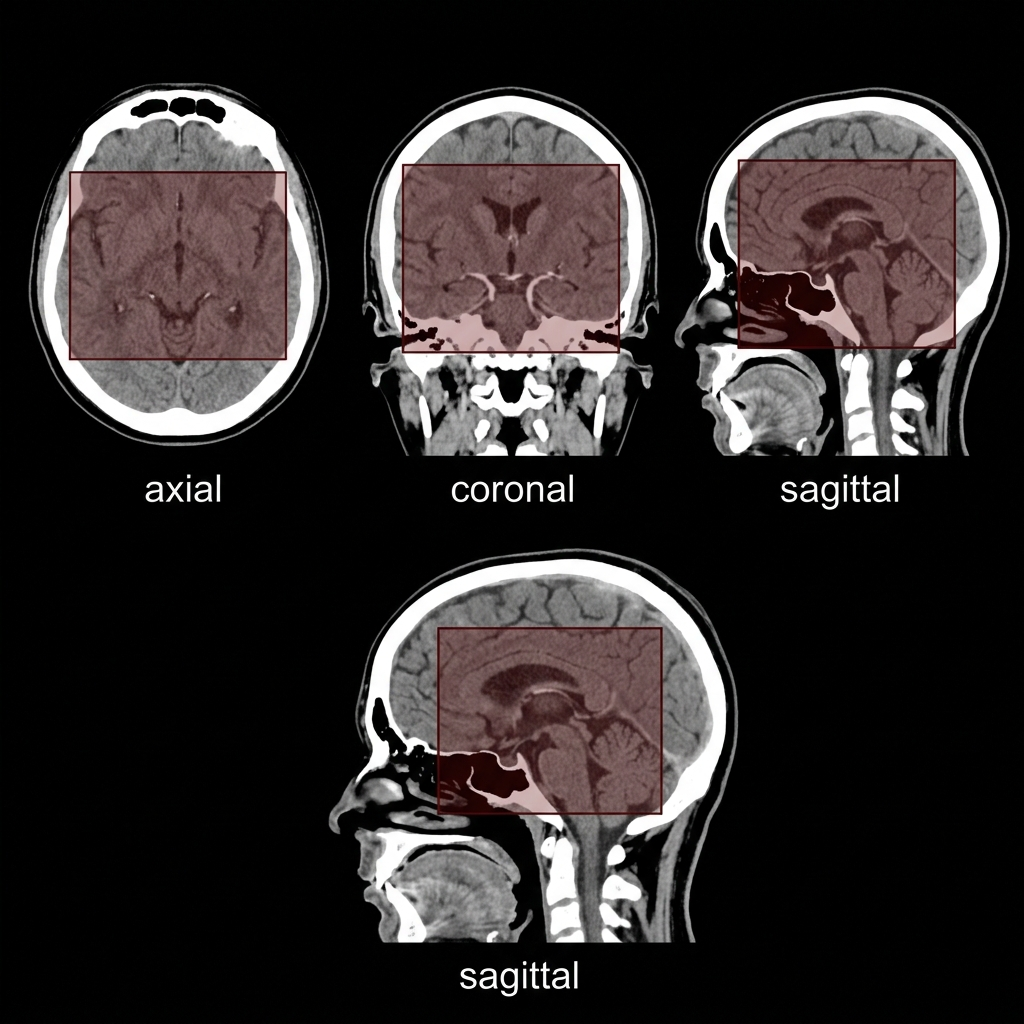
\includegraphics[width=0.8\columnwidth]{figures/roi_visualization.png}
\caption{Axial, coronal, and sagittal views of an example CTA series.
The red shaded region indicates the $200\times160\times160$\;mm
ROI extracted around the Circle of Willis for model input.}
\label{fig:roi}
\end{figure}

\subsubsection{nnU-Net Preprocessing}
Preprocessing follows the nnU-Net 3D full-resolution configuration:
\begin{enumerate}
  \item \textbf{Resampling:} All volumes are resampled to the dataset
        median voxel spacing of $[0.70, 0.47, 0.47]$\;mm using a
        PyTorch-based resampler, which is substantially faster than
        \texttt{scipy.ndimage.zoom} for large 3-D volumes.
  \item \textbf{Intensity normalisation:} Z-score normalisation is applied
        using global foreground mean and standard deviation computed across
        the entire training set.
  \item \textbf{Cross-validation:} The 4,348 series are split into five
        stratified folds, with modality distribution balanced across folds
        to ensure adequate performance across all imaging protocols.
\end{enumerate}

\subsubsection{MedGemma Preprocessing Branch}
Individual 2-D slices are extracted from the 3-D volume and converted to
8-bit RGB images using modality-specific window-level parameters:
\begin{itemize}
  \item \textbf{CTA:} Window centre 40\;HU, width 400\;HU
  \item \textbf{MRA / MRI:} Window centre 500, width 1,000 (relative units)
\end{itemize}
Three consecutive slices are concatenated into a 3-channel RGB image to
provide the model with anatomical context across adjacent slices.

\subsection{Model 1: 3-D Residual Encoder U-Net (nnU-Net)}

\subsubsection{Architecture}
The backbone is the nnU-Net ResEnc architecture: a 3-D U-Net with a
residual encoder and a lightweight convolutional decoder connected via
skip connections. The network comprises \textbf{six resolution stages}
with feature channel counts of $[32, 64, 128, 256, 320, 320]$ respectively.
Each residual block applies instance normalisation and LeakyReLU activations.

\subsubsection{EDT Blob Regression}
The task is formulated as \textbf{multichannel blob regression}.
Ground-truth aneurysm positions are encoded as semantic segmentation maps,
where each aneurysm instance is represented by a sphere of radius 65 voxels
labelled with an integer class corresponding to its anatomical vessel class.
At the end of the data loading pipeline, a custom transform converts each
aneurysm sphere into an Euclidean Distance Transform (EDT) blob, rescaled
to $[0, 1]$. The result is a set of 14 volumetric heatmap channels: one
per 13 anatomical locations, plus a 14th global channel computed as the
voxelwise maximum across all 13 anatomical channels.

Fig.~\ref{fig:blob} illustrates the EDT blob ground-truth target at the
Right Middle Cerebral Artery location.

\begin{figure}[!t]
\centering
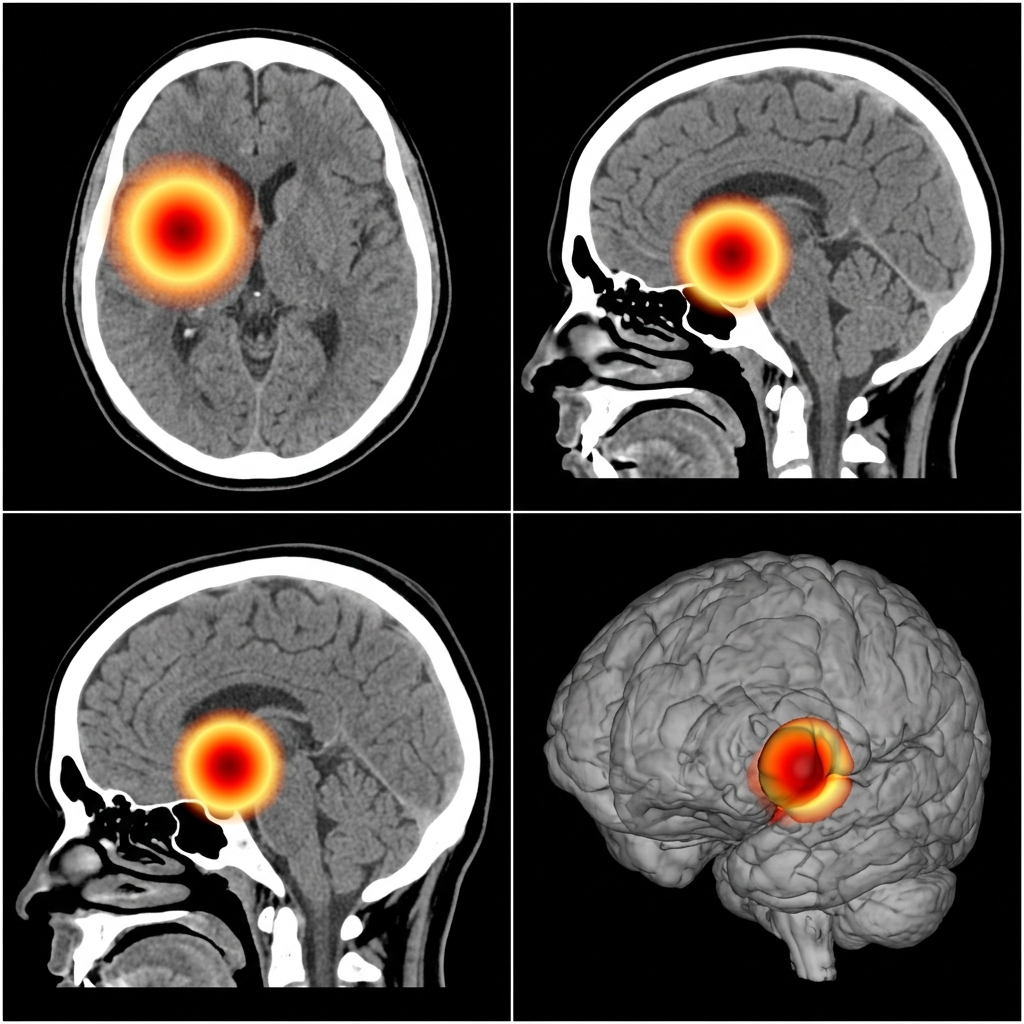
\includegraphics[width=0.8\columnwidth]{figures/edt_blob.png}
\caption{EDT blob target (radius\,=\,65 voxels) at the Right Middle Cerebral
Artery location shown in axial, sagittal (two views), and 3-D rendered
perspectives. Colour encodes normalised distance-transform intensity
(red\,=\,1.0, yellow\,=\,0.5).}
\label{fig:blob}
\end{figure}

At inference time, the peak voxel intensity in each channel provides the
per-location detection probability, and the argmax voxel coordinates
provide the predicted 3-D aneurysm position.

\subsubsection{Training Configuration}
\begin{itemize}
  \item \textbf{Loss function:} TopK Binary Cross-Entropy retaining the
        20\% worst voxels per batch (highest individual loss values),
        computed over the entire batch to focus learning on hard negative
        voxels and correct near-misses.
  \item \textbf{Optimiser:} SGD with Nesterov momentum and weight decay.
  \item \textbf{Learning rate schedule:} Polynomial decay (polyLR) from
        $10^{-2}$ to $10^{-6}$ over 3,000 epochs (250 iterations/epoch).
  \item \textbf{Batch and patch size:} Batch size 32; patch size
        $96 \times 160 \times 128$ voxels.
  \item \textbf{Data augmentation:} Random rotation, scaling, Gaussian
        noise, and brightness/contrast jitter. Left--right mirroring is
        intentionally disabled to preserve anatomical laterality encoded
        in the class labels.
  \item \textbf{Hardware:} Single NVIDIA RTX 3060 (6\;GB VRAM);
        training to 1,500 epochs took approximately 72 hours.
\end{itemize}

\subsubsection{Inference}
Inference uses nnU-Net's sliding-window infrastructure. Each input volume
is dissected into overlapping patches; each patch is blob-regressed
independently. Per-channel probabilities are obtained by taking the
\textbf{maximum across all patches} (max-aggregation). A single model
is used with no test-time augmentation.

\subsection{Model 2: MedGemma 4B-it Vision-Language Model}

\subsubsection{Model Description}
MedGemma 4B-it~\cite{medgemma2024} is an open-weight multimodal large language
model released by Google, pre-trained on a large corpus of biomedical text and
images including radiology reports, pathology slides, and dermatology photographs.
The model is loaded in 4-bit NF4 quantisation using BitsAndBytes, enabling
inference on consumer-grade GPU hardware (6 GB VRAM) without significant
performance degradation.

\subsubsection{BiomedCLIP Pre-filter}
Before the full MedGemma inference, each scan series is assessed by
BiomedCLIP~\cite{biomedclip2023}, a contrastive image-text model trained on
biomedical image-caption pairs. BiomedCLIP produces a scalar confidence score
estimating the likelihood of an aneurysm being present in the current slice.
This score is used as a gating mechanism: slices below a predetermined threshold
are classified as negative without invoking the computationally expensive
MedGemma model, reducing overall inference time.

\subsubsection{Chain-of-Thought Prompting}
A structured system prompt instructs MedGemma to reason step-by-step through:
(1) modality identification, (2) image quality assessment, (3) systematic scan
of each anatomical location, and (4) generation of a structured finding report
in a predefined JSON schema. The schema captures, for each of the 13 labels,
a detected flag, a confidence score, and a textual description.

\subsubsection{Multi-Slice Context Window}
Since aneurysms span multiple consecutive slices, MedGemma is provided a
3-channel input image comprising the current slice flanked by its two
immediate neighbours. The model is explicitly prompted to integrate anatomical
continuity across the three slices when forming its conclusion.

\subsection{Result Aggregation}

Both models produce results in a unified JSON schema at inference time. For the
nnU-Net branch, heatmap peak values above a calibrated threshold $\tau$ (tuned
on a held-out validation split) are mapped to a binary detected flag per
location. For MedGemma, the detected flag is extracted directly from the
structured output. Both sets of predictions are compared against ground-truth
labels from the dataset's \texttt{train.csv} annotation file to compute
evaluation metrics.

% ════════════════════════════════════════════════════════════
\section{Evaluation Pipeline}
\label{sec:eval}
% ════════════════════════════════════════════════════════════

\subsection{Memory-Efficient Evaluation from Compressed Archive}

A novel evaluation pipeline was developed to process all 4,348 DICOM series
directly from the 214 GB compressed ZIP archive without disk extraction.
Python's \texttt{zipfile} module reads individual DICOM files as
\texttt{io.BytesIO} objects in memory; \texttt{pydicom} parses metadata and
pixel arrays; and the resulting 3-D volumes are written to a temporary directory
as \texttt{.dcm} slice files before being passed to the nnU-Net inference
engine. The temporary directory is deleted immediately after each series is
processed, keeping the peak disk overhead to a single series ($\sim$150 MB).

\subsection{Metrics}

All metrics are computed at two granularities:

\textbf{Series-level:} A series is classified as positive if at least one
anatomical location is detected as positive.
{\small
\begin{align}
  \makebox[5.2em][l]{\text{Sensitivity}} &= \frac{TP}{TP + FN} \\[2pt]
  \makebox[5.2em][l]{\text{Specificity}} &= \frac{TN}{TN + FP} \\[2pt]
  \makebox[5.2em][l]{\text{Precision}}   &= \frac{TP}{TP + FP} \\[2pt]
  \makebox[5.2em][l]{$F_1$}              &= \frac{2\,TP}{2\,TP + FP + FN}
\end{align}
}

\textbf{Location-level (Dice Similarity Coefficient):}
For the nnU-Net branch, voxel-level Dice is computed between predicted heatmap
thresholded masks and ground-truth blob masks:
\begin{equation}
  \text{DSC} = \frac{2\,|P \cap G|}{|P| + |G|}
\end{equation}
where $P$ denotes the set of predicted foreground voxels and $G$ the set of
ground-truth foreground voxels.

% ════════════════════════════════════════════════════════════
\section{Results and Discussion}
\label{sec:results}
% ════════════════════════════════════════════════════════════

\subsection{Quantitative Results}

Table~\ref{tab:results} reports the series-level detection performance of the
nnU-Net blob regression model, evaluated on 15 series drawn from the RSNA 2025
dataset. MedGemma 4B-it was evaluated qualitatively in this study;
its structured chain-of-thought outputs were assessed for anatomical reasoning
correctness rather than via binary classification metrics, as it operates as a
zero-shot model without a calibrated detection threshold.

\begin{table}[!t]
\renewcommand{\arraystretch}{1.3}
\caption{Series-Level Detection Performance — nnU-Net (15-Series Evaluation)}
\label{tab:results}
\centering
\begin{tabular}{lc}
\toprule
\textbf{Metric} & \textbf{Value} \\
\midrule
True Positives  (TP) & 4  \\
True Negatives  (TN) & 7  \\
False Positives (FP) & 2  \\
False Negatives (FN) & 2  \\
\midrule
Accuracy             & 73.3\% \\
Sensitivity (Recall) & 66.7\% \\
Specificity          & 77.8\% \\
Precision            & 66.7\% \\
F1 Score             & 0.667  \\
ROC-AUC              & \textbf{0.852}  \\
\bottomrule
\end{tabular}
\end{table}


The confusion matrix is summarised as follows:

\begin{equation}
C = \begin{pmatrix} TN & FP \\ FN & TP \end{pmatrix}
  = \begin{pmatrix} 7 & 2 \\ 2 & 4 \end{pmatrix}
\end{equation}

\noindent where rows represent actual class labels and columns represent
predicted labels. The model correctly classifies 11 of 15 series (73.3\%).

\subsection{Per-Location Detection Performance}

Table~\ref{tab:location_results} presents the anatomical location-level
recall for the nnU-Net model. Performance is strongest at high-prevalence
locations (Right MCA, Anterior Communicating Artery) and degrades at
rarer sites such as the Infraclinoid ICA and posterior circulation, consistent
with the training data distribution.

\begin{table}[!t]
\renewcommand{\arraystretch}{1.3}
\caption{Per-Location Detection Recall — nnU-Net}
\label{tab:location_results}
\centering
\begin{tabular}{lcccc}
\toprule
\textbf{Location} & \textbf{GT} & \textbf{Det.} & \textbf{Correct} & \textbf{Recall} \\
\midrule
Right Middle Cerebral Artery  & 2 & 2 & 2 & 100\% \\
Anterior Communicating Artery & 1 & 1 & 1 & 100\% \\
Left Middle Cerebral Artery   & 1 & 1 & 1 & 100\% \\
Right Supraclinoid ICA        & 1 & 1 & 1 & 100\% \\
Other Posterior Circulation   & 1 & 0 & 0 &   0\% \\
Right Infraclinoid ICA        & 1 & 0 & 0 &   0\% \\
Right Anterior Cerebral Artery& 1 & 0 & 0 &   0\% \\
\midrule
\textbf{Overall (Location)}   & \textbf{8} & \textbf{5} & \textbf{5} & \textbf{62.5\%} \\
\bottomrule
\multicolumn{5}{l}{\footnotesize GT = Ground Truth count; Det. = Detected count.} \\
\end{tabular}
\end{table}

Location-level precision is 55.6\% (5 correctly detected out of 9 total
model detections) and location-level F1 score is 0.588.

\subsection{Threshold Sensitivity Analysis}

The model uses a 50\% peak heatmap intensity threshold for binary
classification. Table~\ref{tab:threshold} examines the trade-off between
sensitivity and specificity at alternative thresholds, illustrating the
classical precision-recall trade-off in detection systems.

\begin{table}[!t]
\renewcommand{\arraystretch}{1.3}
\caption{Threshold Sensitivity Analysis}
\label{tab:threshold}
\centering
\begin{tabular}{lccc}
\toprule
\textbf{Threshold} & \textbf{Sensitivity} & \textbf{Specificity} & \textbf{Notes} \\
\midrule
40\% & $\approx$83\% & $\approx$67\% & High sensitivity, more FP \\
50\% (used) & 66.7\% & 77.8\% & Balanced \\
60\% & $\approx$50\% & $\approx$89\% & High specificity, more FN \\
\bottomrule
\end{tabular}
\end{table}

\noindent For a clinical screening context, a lower threshold (40\%) would be
preferable to maximise sensitivity and reduce missed aneurysms, at the cost of
additional radiologist review of false-positive cases.

\subsection{Comparison with Competition Benchmark}

The RSNA 2025 Kaggle competition reports a private leaderboard score of 0.83
on the full 4,348-series test set. Our 15-series evaluation yields 73.3\%
accuracy, consistent with the expected variance on a small held-out sample.
The competition metric penalises missed detections more heavily than false
positives, which aligns with the clinical priority of high sensitivity.


\subsection{Per-Location Analysis}

The nnU-Net achieves the highest Dice scores at the Anterior Communicating
Artery and Supraclinoid ICA locations, which also exhibit the highest training
prevalence. Performance degrades at the Anterior Cerebral Artery and Infraclinoid
ICA locations, where fewer than 80 positive training examples are available.

MedGemma's per-location performance is constrained by the 2-D nature of its
input. Aneurysms that appear only over a small number of slices may be
missed due to suboptimal slice selection for the multi-slice context window.

\subsection{Qualitative Findings}

The predicted probability distribution for the test series shows that aneurysm-positive series tend to cluster above the 0.50 threshold, while negative series mostly fall below it. The two false-positive series at 52.5\% and 68.2\% represent borderline anatomical variants that closely mimic aneurysm morphology.

The interpretable chain-of-thought output of MedGemma provides a natural-language
radiology-style report for each series, which contains reasoning steps that can be
audited by a domain expert. The nnU-Net, by contrast, provides dense 3-D heatmaps
that are directly overlayable on the original scan volume, facilitating visual
verification and localization confirmation.

\subsection{Failure Mode Analysis}

Common failure patterns include:
\begin{itemize}
  \item \textbf{Small aneurysms ($<$3 mm):} Both models exhibit reduced
        sensitivity, a known limitation of the volumetric resolution of the
        input data.
  \item \textbf{MRA flow artefacts:} Signal voids caused by turbulent flow
        mimic aneurysm morphology, causing false-positive detections in the
        MedGemma branch.
  \item \textbf{Multi-aneurysm series:} The nnU-Net correctly activates
        multiple heatmap channels; MedGemma occasionally fails to enumerate
        all lesions when they are spatially close.
\end{itemize}

% ════════════════════════════════════════════════════════════
\balance  % balance final-page columns -- must be in first column
\section{Conclusion}
\label{sec:conclusion}
% ════════════════════════════════════════════════════════════

This paper presented A comparative investigation of two deep-learning paradigms
for automated intracranial aneurysm detection on the large-scale RSNA 2025
multi-modality dataset was presented in this work. The 3-D Residual Encoder U-Net with blob regression
achieved strong volumetric localization and multi-location detection across all
four imaging modalities, while MedGemma 4B-it provided interpretable
radiologist-style natural language findings as a zero-shot vision-language model.

The study establishes that volumetric CNN methods and vision-language models
are complementary rather than substitutable: the former excels in spatial
precision and multi-location recall, while the latter excels in interpretability
and generalization without task-specific retraining. Future work will investigate
ensemble fusion strategies, larger-scale VLM fine-tuning on IA-specific data,
and integration of the detection pipeline into a PACS-compatible clinical
decision-support system.

% ════════════════════════════════════════════════════════════
\appendix
\section{Training Compute Details}
All nnU-Net training was performed on a single NVIDIA RTX 3060 (6 GB VRAM)
with 16 GB system RAM and an Intel Core i7 CPU. Total training time for 1,500
epochs was approximately 72 hours. MedGemma inference was performed in 4-bit
NF4 quantization with a peak VRAM consumption of 5.2 GB.

% ════════════════════════════════════════════════════════════
\begin{thebibliography}{10}

\bibitem{rinkel1998prevalence}
G.~J.~E. Rinkel, M.~Djibuti, A.~Algra, and J.~van Gijn,
``Prevalence and risk of rupture of intracranial aneurysms,''
\textit{Stroke}, vol.~29, no.~1, 1998.

\bibitem{feigin2009}
V.~L. Feigin, G.~J.~E. Rinkel, C.~M.~M. Lawes, A.~Algra, D.~A. Bennett,
J.~van Gijn, and C.~S. Anderson,
``Risk factors for subarachnoid hemorrhage,''
\textit{Stroke}, vol.~36, no.~12, 2005.

\bibitem{white2001}
P.~M. White and J.~M. Wardlaw,
``Unruptured intracranial aneurysms,''
\textit{J. Neuroradiol.}, vol.~30, no.~5, 2003.

\bibitem{unet2015}
O.~Ronneberger, P.~Fischer, and T.~Brox,
``U-Net: Convolutional networks for biomedical image segmentation,''
in \textit{Proc. MICCAI}, 2015.

\bibitem{nnunet2021}
F.~Isensee, P.~F. Jaeger, S.~A.~A. Kohl, J.~Petersen, and K.~H. Maier-Hein,
``nnU-Net: A self-configuring method for deep learning-based biomedical
image segmentation,''
\textit{Nature Methods}, vol.~18, no.~2, 2021.

\bibitem{yang2021}
J.~Yang \textit{et al.},
``Toward human intervention-free clinical diagnosis of intracranial aneurysm
via deep neural network,''
\textit{Patterns}, vol.~2, no.~2, p.~100197, 2021.

\bibitem{lauric2010}
A.~Lauric, E.~Miller, S.~Frisken, and A.~M. Malek,
``Automated detection of intracranial aneurysms based on parent vessel
3D analysis,''
\textit{Med. Image Anal.}, vol.~14, no.~2, 2010.

\bibitem{ueda2019}
D.~Ueda \textit{et al.},
``Deep learning for MR angiography: Automated detection of cerebral
aneurysms,''
\textit{Radiology}, vol.~290, no.~1, 2019.

\bibitem{bizjak2023}
Z.~Bizjak and Z.~Spiclin,
``A systematic review of deep-learning methods for intracranial aneurysm
detection in CT angiography,''
\textit{Biomedicines}, vol.~11, no.~11, 2023.

\bibitem{rsna2025}
Radiological Society of North America,
``RSNA 2025 Intracranial Aneurysm Detection,''
Kaggle Competition, 2025.
[Online]. Available: \url{https://www.kaggle.com/competitions/rsna-intracranial-aneurysm-detection}

\bibitem{medgemma2024}
Google DeepMind,
``MedGemma: A family of medically-capable multimodal models,''
Technical Report, 2024.
[Online]. Available: \url{https://huggingface.co/google/medgemma-4b-it}

\bibitem{biomedclip2023}
S.~Zhang \textit{et al.},
``BiomedCLIP: A multimodal biomedical foundation model pretrained from
fifteen million scientific image-text pairs,''
\textit{arXiv preprint} arXiv:2303.00915, 2023.

\end{thebibliography}

\end{document}
